\documentclass[border=10pt]{standalone}

\usepackage{tikz}
\usepackage{tikzsymbols}
\usetikzlibrary{calc,patterns,shapes.geometric}

\def\centerarc[#1](#2)(#3:#4:#5){\draw[#1] ($(#2)+({#5*cos(#3)},{#5*sin(#3)})$) arc (#3:#4:#5);}

\begin{document}
	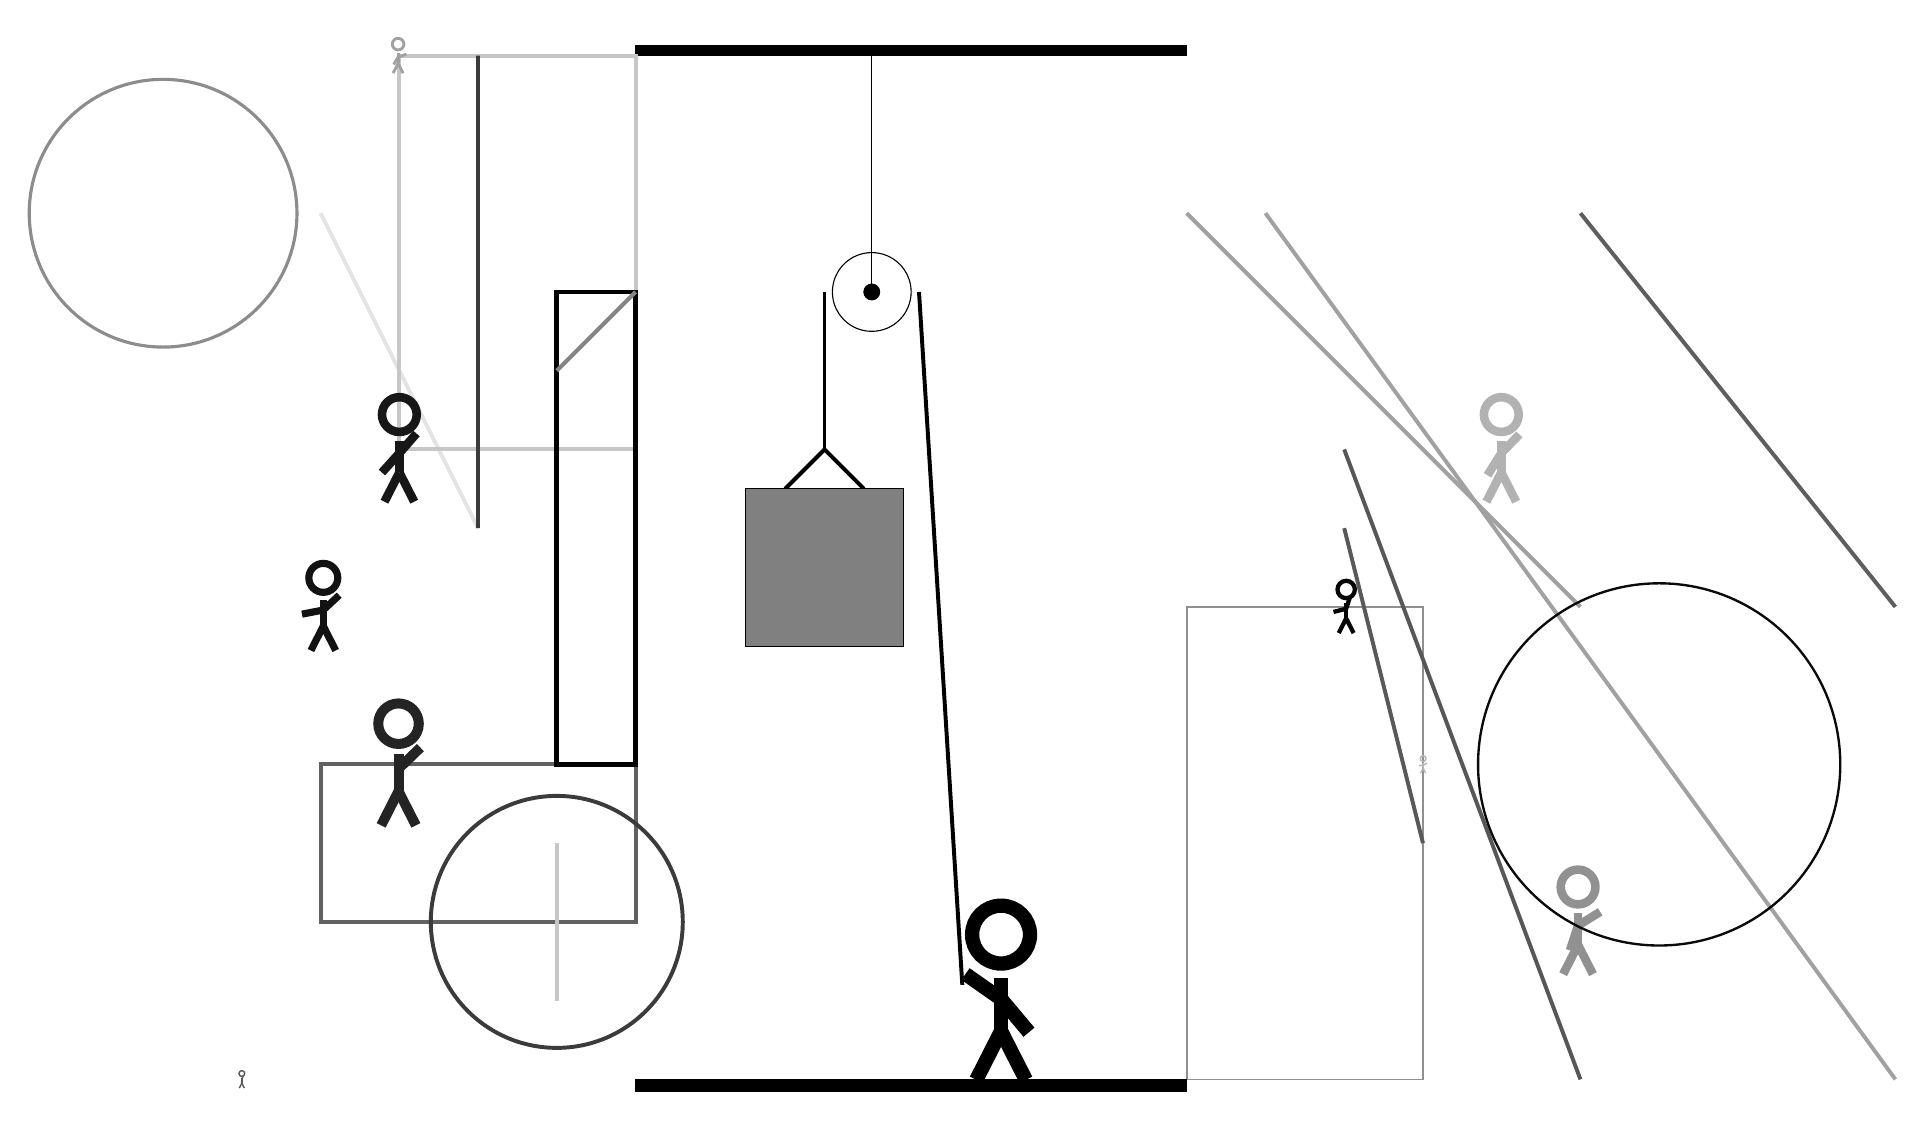
\begin{tikzpicture}
		%%%%% START %%%%%
		
		\draw[fill=black] (-2, 10) rectangle (5, 10.125);
		
		\draw (1, 7) circle (0.5);
		\draw[fill=black] (1, 7) circle (0.1);
		\draw (1, 10) -- (1, 7);
		
		\draw[line width=0.5mm] (-0.1, 4.5) -- (0.4, 5.0) -- (0.9, 4.5);
		\draw[fill=black!50] (-0.6, 4.5) rectangle (1.4, 2.5);
		
		\draw[line width=0.5mm] (0.4, 7) -- (0.4, 5.0);
		\centerarc[line width=0.5mm](1, 7)(0:180:0.6);
		\draw[line width=0.5mm](1.6, 7) -- (2.15, -1.8);
		
		\draw[line width=0.5mm, color=black!34](-2, 4) -- (-2, 3);
		
		\draw[line width=0.5mm, color=black!11](-4, 4) -- (-6, 8);
		\draw[line width=0.2mm, color=black!44] (5, -3) rectangle (8, 3);
		\node[line width=0.2mm, color=black!43] at (10, -1) {\Strichmaxerl[6][72][32]};
		\draw[line width=0.5mm, color=black!22] (-2, 5) rectangle (-5, 10);
		
		\draw[line width=0.5mm, color=black!37](6, 8) -- (14, -3);
		\draw[line width=0.5mm, color=black!63](10, 8) -- (14, 3);
		\draw[line width=0.5mm, color=black!37](5, 8) -- (10, 3);
		\node[line width=0.4mm, color=black!93] at (-6, 3) {\Strichmaxerl[5][11][43]};
		\draw [line width=0.4mm, color=black!45](-8, 8) circle (1.7);
		\draw[line width=0.5mm, color=black!62] (-2, 1) rectangle (-6, -1);
		\draw [line width=0.5mm, color=black!77](-3, -1) circle (1.6);
		\node[line width=0.3mm, color=black!91] at (-5, 5) {\Strichmaxerl[6][48][49]};
		
		\node[line width=0.3mm, color=black!65] at (-7, -3) {\Strichmaxerl[1][86][73]};
		\draw[line width=0.6mm, color=black!77] (-4, 10) rectangle (-4, 4);
		\node[line width=0.6mm, color=black!98] at (7, 3) {\Strichmaxerl[3][14][72]};
		
		\node[line width=0.7mm, color=black!30] at (9, 5) {\Strichmaxerl[6][58][46]};
		\draw[line width=0.5mm, color=black!66](10, -3) -- (7, 5);
		\draw[line width=0.6mm, color=black!99] (-2, 7) rectangle (-3, 1);
		
		\node[line width=0.4mm, color=black!37] at (-5, 10) {\Strichmaxerl[2][60][18]};
		\draw[line width=0.5mm, color=black!22](-3, -2) -- (-3, 0);
		
		\node[line width=0.2mm, color=black!86] at (-5, 1) {\Strichmaxerl[7][90][44]};
		
		\node[line width=0.4mm, color=black!29] at (8, 1) {\Strichmaxerl[1][10][26]};
		\draw[line width=0.5mm, color=black!65](7, 4) -- (8, 0);
		\draw [line width=0.3mm, color=black!96](11, 1) circle (2.3);
		
		\draw[line width=0.5mm, color=black!48](-3, 6) -- (-2, 7);
		
		\node at (2.6, -1.9) {\Strichmaxerl[10][-35][-50]};
		
		\draw[fill=black] (-2, -3) rectangle (5, -3.15);
		
		%%%%% END %%%%%
	\end{tikzpicture}
\end{document}